%課題研究レジュメテンプレート ver. 1.2

\documentclass[uplatex]{jsarticle}
\usepackage[top=20mm,bottom=20mm,left=20mm,right=20mm]{geometry}
\usepackage[T1]{fontenc}
\usepackage{txfonts}
\usepackage{wrapfig}
\usepackage[expert,deluxe]{otf}
\usepackage[dvipdfmx,hiresbb]{graphicx}
\usepackage[dvipdfmx]{hyperref}
\usepackage{pxjahyper}
\usepackage{secdot}

\makeatletter
  \renewcommand{\section}{%
    \if@slide\clearpage\fi
    \@startsection{section}{1}{\z@}%
    {\Cvs \@plus.5\Cdp \@minus.2\Cdp}% 前アキ
    {.5\Cvs \@plus.3\Cdp}% 後アキ
    %{\normalfont\Large\headfont\raggedright}}
    {\normalfont\raggedright}}

  \renewcommand{\subsection}{\@startsection{subsection}{2}{\z@}%
    {\Cvs \@plus.5\Cdp \@minus.2\Cdp}% 前アキ
    {.5\Cvs \@plus.3\Cdp}% 後アキ
    %{\normalfont\large\headfont}}
    {\normalfont}}

  \renewcommand{\subsubsection}{\@startsection{subsubsection}{3}{\z@}%
    {\Cvs \@plus.5\Cdp \@minus.2\Cdp}%
    {\z@}%
    %{\normalfont\normalsize\headfont}}
    {\normalfont}}
\makeatother
%ここから上を編集する必要はない.





\title{\vspace{-14mm}アニメ作品の原作の種類とその数の推移}
\author{PMコース 矢吹研究室 1342073 杉山 喜彦}
\date{}%日付を入れる必要はない.
\pagestyle{empty}%ページ番号は振らない.
\begin{document}
\maketitle

\section{研究の背景}

この3年間ほどでネットに上がっていた小説をアニメ化することが多くなってきている.今年の地上波放送されたアニメで「ダンジョンに出会いを求めるのは間違っているだろうか」という作品が放送された.この作品はもともと「小説家になろう」に上げられた作品をGA文庫が引き抜き文庫化の後にアニメ放送されたものだ.他の例としては,「ソードアート・オンライン」,「魔法科高校の劣等生」,「ログ・ホライゾン」などが挙げられる.\par 
ネットの小説をアニメ作品の原作にする事はアニメ作品の原作をネットに上がっていた小説で作成するように移り変わってきたためだと私は考えた.この移り変わりはどのようなものか.どのようにしてアニメ作品の原作が年によって数が変わっていったか.この結果から,次の年でどのアニメ作品の原作の種類が多くなるのかを予測できるのではないかと私は考えた.そこで私は年別で地上波放送されたアニメ作品の原作を調べ,種類別に分けることにした.

\section{研究の目的}

私は地上波放送されたアニメ作品の原作を調べ種類分けをする.次に年別によるアニメ作品の原作の種類別で見た場合の流れとその数の推移をグラフに表示する.このグラフの結果からアニメ作品の原作の種類と推移を考察することが目的である.

\section{プロジェクトマネジメントとの関連}

プロジェクトマネジメントの関連としては,プロジェクト・ステークホルダー・マネジメントと関連性があると考える.この研究はアニメ作品の原作の種類を年別に分け移り変わりを調べているため,次の年で多くなると予想される原作を知ることができるからである.

\section{研究の方法}

本研究では,サイトやwikipediaなどからデータを収集しグラフを作成し考察する.\par 
データの内容として,アニメの放送時間,アニメの名前,アニメ作品の原作の種類,アニメ作品の終了日,原作名,放送時間時期,アニメ作品の長さ,監督名,アニメーション会社,話数,放送局ごとの放送時間である.これらのデータの中からアニメの放送時間,アニメの名前,アニメ作品の原作の種類の三つを用いて以下のように研究を進める.

\begin{enumerate}
\item 年別にアニメ作品をインターネットなどを使って調べる\cite{self01}\cite{self02}\cite{self03}.
\item アニメ作品の原作を調べる\cite{self04}.
\item 調べたデータをエクセルで保存する.
\item アニメ作品の原作を種類分けする.
\item 種類分けしたデータの数をとっていく.
\item これを年別で行う.
\item 種類別でだした数を年別で比較できるようにする.
\item 比較しているグラフを製作する.
\item そのグラフからどのようにアニメ作品の原作が移り変わってきたかを考察する.
\end{enumerate}
\section{現在の進捗状況}
 \begin{wrapfigure}[15]{r}{11cm}
\vspace*{-\intextsep}
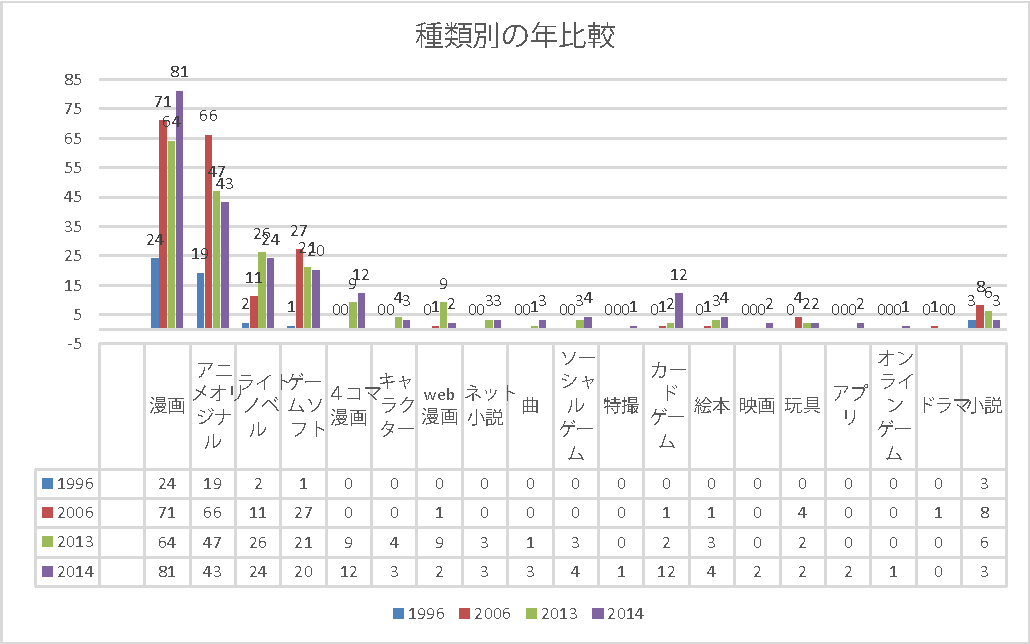
\includegraphics[width=11cm,clip]{01.pdf}
\caption{アニメ作品の原作の種類と数の推移}\label{図1}
\end{wrapfigure}
グラフを見てから分かったことは,漫画は年々1位だが2006年と2013年の間で下がり,次の2014年の漫画は64作品から81作品と17作品増えていたことが分かった.二つ目に分かったことは,他の種類のアニメオリジナル,ライトノベル,ゲームソフトがだんだんと下がってきていることも分かった.三つ目に分かったことは1996年と2006年でのアニメ作品の原作の種類が10種類に対し2013年と2014年では18種類に増えていることが分かった.\par 
\par 
以下のものはアニメ作品の原作の種類を年別でランキング3位まで出したものである\par
 ※原作の種類(その年の作品数)\par 
1996年  1位は漫画(24)   2位はアニメオリジナル(19)  3位は小説(3)\par 
2006年  1位は漫画(71)   2位はアニメオリジナル(66)  3位はゲームソフト(27)\par 
2013年  1位は漫画(64)   2位はアニメオリジナル(47)  3位はライトノベル(26)\par
2014年  1位は漫画(81)   2位はアニメオリジナル(43)  3位はライトノベル(24)\par

\section{今後の計画}
今後,抜けている年アニメ作品の原作の種類とその数の推移のデータを集めて1996年から2015年までのグラフを作成する.出来上がったグラフからアニメ作品の原作の種類とその数の推移から移り変わりを考察する.次の年のアニメ作品の原作の種類とその数の推移を予測する事を目標とする.\par
以下のように研究を進める.
\begin{enumerate}
\item 抜けている年のデータと集めきれなかったデータを集める.
\item 集めたデータをエクセルで保存し,グラフに追加する.
\item 今までのアニメ作品の原作の種類とその数の推移から次の年のアニメ作品の原作の種類とその数の推移を予測する.
\end{enumerate}

\bibliographystyle{junsrt}
\bibliography{biblio}%「biblio.bib」というファイルが必要.

\end{document}